%%%%%%%%%%%%%%%%%%%%%%%%%%%%%%%%%%%%%%%%%%%%%%%%%%%%%%%%%%%
% --------------------------------------------------------
% Tau
% LaTeX Template
% Version 2.4.3 (01/09/2024)
%
% Author: 
% Guillermo Jimenez (memo.notess1@gmail.com)
% 
% License:
% Creative Commons CC BY 4.0
% --------------------------------------------------------
%%%%%%%%%%%%%%%%%%%%%%%%%%%%%%%%%%%%%%%%%%%%%%%%%%%%%%%%%%%

\documentclass[9pt,a4paper,twoside]{tau-class/tau}
\usepackage[english]{babel}

%----------------------------------------------------------
% TITLE
%----------------------------------------------------------

\journalname{Fundamentals of Natural Language Processing}
%% TODO: Optional, you can set a fancier title if you like
\title{Negation and Uncertainty Detection using Classical and Machine Learning Techniques}

%----------------------------------------------------------
% AUTHORS, AFFILIATIONS AND PROFESSOR
%----------------------------------------------------------

%% TODO: Set your names here
\author[a,1]{Author One}
\author[b,2]{Author Two}
\author[c,3]{Author Three}
\author[d,4]{Author Four}

%----------------------------------------------------------

\affil[a]{NIU of Author one}
\affil[b]{NIU of author two}
\affil[c]{NIU of author three}
\affil[d]{NIU of author four}

%----------------------------------------------------------
% FOOTER INFORMATION
%----------------------------------------------------------

\institution{Universitat Autònoma de Barcelona}
\footinfo{Class Project}
\theday{July 26, 2024}
\leadauthor{Group XX} 		%% TODO: Set your group ID here
\course{Fundamentals of Natural Language Processing}

%----------------------------------------------------------
% ABSTRACT AND KEYWORDS
%----------------------------------------------------------

\begin{abstract}    
	%% TODO: Change this default abstract into something nice that describes your work.
	%% Keep it below 300 words.
    An abstract is a brief summary that outlines the key aspects of a work. An example of a famous abstract is reproduced verbatim here for illustration purposes \cite{vaswani_attention_2017}: The dominant sequence transduction models are based on complex recurrent or convolutional neural networks that include an encoder and a decoder. The best performing models also connect the encoder and decoder through an attention mechanism. We propose a new simple network architecture, the Transformer, based solely on attention mechanisms, dispensing with recurrence and convolutions entirely. Experiments on two machine translation tasks show these models to be superior in quality while being more parallelizable and requiring significantly less time to train. Our model achieves 28.4 BLEU on the WMT 2014 Englishto-German translation task, improving over the existing best results.
\end{abstract}

%----------------------------------------------------------

%% TODO: Set appropriate keywords for your report.
\keywords{a, b, c, d}

%----------------------------------------------------------

\begin{document}
	%% Do NOT change any of this. Line numbers should be kept.
    \maketitle 
    \thispagestyle{firststyle} \tauabstract 
    \tableofcontents
    \linenumbers 
    
%----------------------------------------------------------

\section{Introduction}

    \taustart{T}his sample document contains indications about how to write the report for the project in the subject of Natural Language Processing. The full report must be no longer than 5 pages without including references. \textbf{Any additional pages will not be evaluated}. The section structure is open, but you are encouraged to follow a principled academic writing style (you may mimic that of the papers provided as references). \textbf{Form will be taken into account in the evaluation of the project.}

\section{Writing \LaTeX}

	\LaTeX is the typesetting tool that most academics use these days. For this reason, you are required to present your work using it. \LaTeX has a bit of a steep learning curve at the beginning, but you will see that it is quite intuitive and you will get progressively more productive at it as you write.

    \subsection{Basics}

    \LaTeX is based on the idea of defining commands (or macros) that control the presentation of the text on a document. As a matter of fact, \LaTeX ignores whitespace except for double newlines (pressing intro twice), which is used to delimit paragraphs. Commands are usually preceeded by a backslash (\\) and have a number of arguments, if any, between braces (\{ and \}). You can set a \textbf{bold} or an \textit{italic} typeface using the \verb|\textbf{.}| and \verb|\textit{.}| commands. You can also {\tiny change the size of the font for a scope}. You can change {\color{red} text color} using the \verb|\color{col}| command. 

    Nevertheless, you should mostly refrain from formatting text explicitly. \LaTeX provides commands for recurring types of  text modifications with some batteries included. For instance, if you want to divide your text in chunks under prominent titles you can use the \verb|\section{.}|, \verb|\subsection{.}|, \verb|\subsubsection{.}| ... etc commands, which will handle everything for you. These titles will automatically appear in the table of contents, they will be properly numbered in the order of appearance, etc. If you are writing a book, you can also use the \verb|\part{.}| and \verb|\chapter{.}| commands for this.

    Many \LaTeX constructs are built around the \verb|\begin{environment}| and \verb|\end{environment}| commands. You write some text between these two commands that is to be formatted according to the rules of the given environment. With this, you can write

    \begin{itemize}
        \item Bullet point lists (environment itemize)
    \end{itemize}

    \begin{enumerate}
        \item Enumerations (environment enumerate)
    \end{enumerate}

    \begin{info}
        ... or some custom stuff as well. The possibilities are quite endless, really.
    \end{info}

    You can edit \LaTeX in any text editor of your choice. I suggest that you try \href{https://www.overleaf.com/}{Overleaf} first, because the editing experience is very simple and very close to that of a shared Google Docs. These days they have gotten quite stingy however, so I suggest using VS Code with the \LaTeX Workshop extension instead. If you need to share the document, just put it in a Git repository. There are a myriad alternatives, so go out there and try what works for you.
		
\section{Figures and tables} \label{sec:table}

    \subsection{Figures}
		
	Fig. \ref{fig:figure} shows an example figure. Figures can be referenced using \verb|\ref{ident}|, where \texttt{name} is a previously-defined \verb|\label{name}| for any object in the document. You can actually also do this with sections (Section \ref{sec:table}) or equations or other types of objects that will be seen below.
		
	\begin{figure}[H]
		\centering
		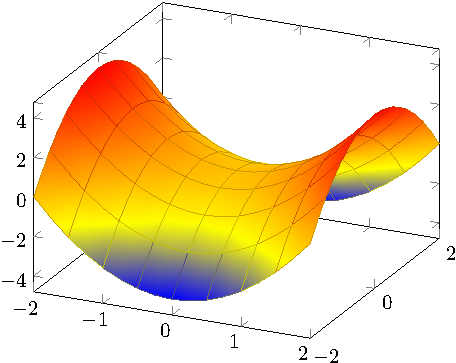
\includegraphics[width=0.75\columnwidth]{Example.pdf}
		\caption{Example figure obtained from PGFPlots \cite{PFGPlots}.}
		\label{fig:figure}
	\end{figure}
		
        Fig. \ref{fig:examplefloat} shows an example of two figures that cover the width of the page. It can be placed at the top or bottom of the page. The space between the figures can also be changed using the \verb|\hspace{Xpt}| command.
		
        \begin{figure*}[tp] % t for position at the top of the current page; b for position at the bottom; p for new page
		\centering
		  \begin{subfigure}[b]{0.38\linewidth} % Fig (a)
			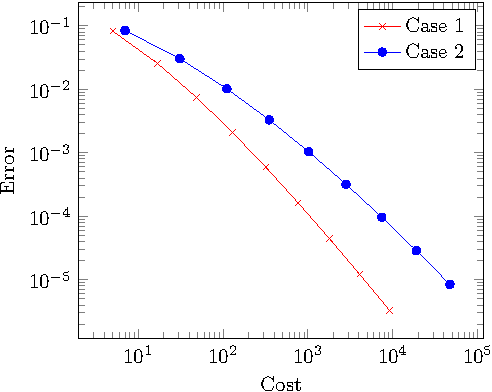
\includegraphics[width=\linewidth]{Example2.pdf}
			\caption{Example left figure.}
			\label{fig:figa}
		\end{subfigure}
			\hspace{20pt}   % Space between the figures
		\begin{subfigure}[b]{0.375\linewidth} % Fig (b)
			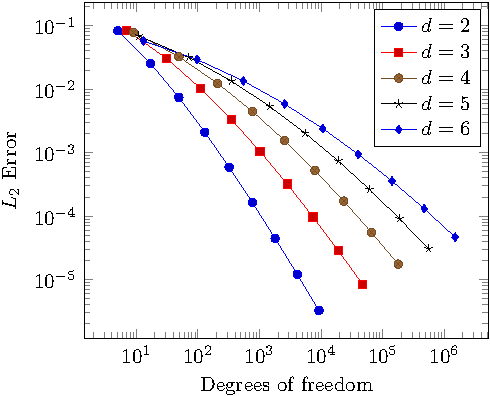
\includegraphics[width=\linewidth]{Example3.pdf}
			\caption{Example right figure.}
			\label{fig:figb}
		\end{subfigure}
		\caption{Example figure that covers the width of the page obtained from PGFPlots \cite{PFGPlots}.}
		\label{fig:examplefloat}
	\end{figure*}

    \begin{info}
    	Figures in \LaTeX are known to be quite anarchic. You should always wait until the very end to place them well into the document. In any case, you should always reference the Figure and provide a Caption so that it can be contextualised even when it lies far away from the text that accompanies it.
    \end{info}

    \begin{info}
    	Avoid raster graphics (jpeg, png) for figures if you can. Always use vectorial formats for plots and diagrams. The preferred formats for vectorial images are SVGs converted to Encapsulated Post-Script (.eps, you can use Inkscape to perform this conversion) or PDF files. Regardless of the image format you are using, generate reasonably high-resolution files (the usual is 300dpi, which means 300 pixels per squared inch). \textbf{Keep in mind that Matplotlib can be configured to generate plots with these settings.}
    \end{info}

    \subsection{Tables}
	
        Table \ref{tab:table} shows an example table. The \verb|\tabletext{}| is used to add notes to tables easily. 

        \begin{info}
        	This template uses the \texttt{booktabs} package by default. This package makes typesetting nice tables easier, but it imposes some general design guidelines. The most prominent is the distinction between middle and edge rules (horizontal lines) and the discouragement of vertical lines.
        \end{info}

        \begin{info}
        	You should \textbf{always} avoid typesetting tables by hand. Use tools such as \href{https://www.tablesgenerator.com/}{this one} to spare yourself some unnecessary pain.
        \end{info}
		
	\begin{table}[H]
		\centering
		\caption{Small example table.}
		\label{tab:table}
		\begin{tabular}{cc}
			\toprule
			\textbf{Column 1} & \textbf{Column 2} \\
			\midrule
			Data 1 & Data 2 \\
			Data 3 & Data 4 \\
			\bottomrule
		\end{tabular}
			
            \tabletext{Note: I'm a table text for additional information.}
			
	\end{table}
		
\section{Tau packages}

    \subsection{Tauenvs}
	
        This template has its own environment package \textit{tauenvs.sty} designed to enhance the presentation of the document. Among these custom environments are \textit{tauenv}, \textit{info} and \textit{note}.
		
        There are two environments which have a predefined title. These can be included by the command \verb|\begin{note}| and \verb|\begin{info}|. All the environments have the same style.
			
        An example using the tau environment is shown below.
		
	\begin{tauenv}[frametitle=Environment with custom title]
            This is an example of the custom title environment. To add a title type \verb|[frametitle=Your title]| next to the beginning of the environment (as shown in this example).
	\end{tauenv}
		
        Tauenv is the only environment that you can customize its title. On the other hand, info and note adapt their title to Spanish automatically when this language package is defined.
		
    \subsection{Taubabel}

        In this new version, we have included a package called \textit{taubabel}, which have all the commands that automatically translate from English to Spanish when this language package is defined. 
        
        By default, tau displays its content in English. However, at the beginning of the document you will find a recommendation when writing in Spanish. 
		
        \textit{Note:} You may modify this package if you want to use other language than English or Spanish. This will make easier to translate the document without having to modify the class document.
		
\section{Equation}

    Equation \ref{ec:equation}, shows the Schrödinger equation as an example. 
	\begin{equation} \label{ec:equation}
		\frac{\hbar^2}{2m}\nabla^2\Psi + V(\mathbf{r})\Psi = -i\hbar \frac{\partial\Psi}{\partial t}
	\end{equation} 
    The \textit{amssymb} package was not necessary to include, because stix2 font incorporates mathematical symbols for writing quality equations. In case you choose another font, uncomment this package in tau-class/tau.cls/math packages.
	
    If you want to change the values that adjust the spacing above and below the equations, play with \verb|\setlength{\eqskip}{8pt}| value until the preferred spacing is set.
	
\section{Adding codes}
	
    This class\footnote{Hello there! I am a footnote :)} includes the \textit{listings} package, which offers customized features for adding codes in \LaTeX\ documents specifically for C, C++, \LaTeX\ and Matlab. 
	
    You can customize the format in tau-class/tau.cls/listings style.
	
        \nolinenumbers
            \lstinputlisting[caption=Example of Matlab code., language=Matlab,label=code]{example.m}
	\linenumbers
	
    If line numbering is defined at the beginning of the document, I recommend placing the command \verb|\nolinenumbers| at the start and \verb|\linenumbers| at the end of the code. 
	
    This will temporarily remove line numbering and the code will look better as shown in Code \ref{code}.
	
\section{References}

    The default formatting for references follows the IEEE style. You can modify the style of your references, for that, go to tau-class/tau.cls/biblatex. See appendix for more information.
	
\section{Appendix}

    \subsection{Alternative title}

        You can make the following modification in tau-class/tau.cls/title preferences section to change the position of the title.

\nolinenumbers
\begin{lstlisting}[language=TeX, caption=Alternative title.]
\newcommand{\titlepos}{\centering}
\end{lstlisting}
\linenumbers

	This will move the title to the center. 

    \subsection{Info environment}

        An example of the info environment declared in the ‘tauenvs.sty’ package is shown below. Remember that \textit{info} and \textit{note} are the only packages that translate their title (English or Spanish).
		
	\begin{info}
		Small example of info environment.
	\end{info}

    \subsection{Equation skip value}

        With the \verb|\eqskip| command you can change the spacing for equations. The default \textit{eqskip} value is 8pt.

\nolinenumbers
\begin{lstlisting}[language=TeX, caption=Equation skip code.]
\newlength{\eqskip}\setlength{\eqskip}{8pt}
	\expandafter\def\expandafter\normalsize\expandafter{%
		\normalsize%
		\setlength\abovedisplayskip{\eqskip}%
		\setlength\belowdisplayskip{\eqskip}%
		\setlength\abovedisplayshortskip{\eqskip-\baselineskip}%
		\setlength\belowdisplayshortskip{\eqskip}%
	}
\end{lstlisting}
\linenumbers
		
    \subsection{References}
		
        In case you require another reference style, you can go to tau-class/tau.cls/biblatex and modify the following.
		
\nolinenumbers
\begin{lstlisting}[language=TeX, caption=References style.]
\RequirePackage[
	backend=biber,
	style=ieee,
	sorting=ynt
]{biblatex}
\end{lstlisting}
\linenumbers

        By default, \textit{tau class} has its own .bib for this example, if you want to name your own bib file, change the \textit{addbibresource}.
		
\nolinenumbers
\begin{lstlisting}[language=TeX]
\addbibresource{tau.bib}
\end{lstlisting}
\linenumbers

\section{Acknowledgements}

Tau \LaTeX template built by Guillermo Jimenez.

%----------------------------------------------------------

\addcontentsline{toc}{section}{References}
\printbibliography

%----------------------------------------------------------

\end{document}